% -*- coding: UTF-8 -*-
% hurlex-chapt7.tex
% hurlex 开发文档 第7章内容

\section {添加中断描述符表}

\subsection{中断的引入}

\par 中断是用以提高计算机工作效率、增强计算机功能的一项重要技术。其实简单说中断就是一种通知机制罢了。我们知道操作系统的一个\allowbreak
核心任务就是和连接在主板上的所有的硬件设备进行通信,但是CPU和这些外设的速率根本就不在一个数量级上,倘若CPU向某一个设备发出一\allowbreak
个请求并且一直等待反馈结果的话,这样带来的性能损失是不可接受的。而且CPU在运行期间需要得知外设所发生的事件,轮询显然是不可取\allowbreak
的,那么就迫切需要一种机制来帮助我们解决这个问题。

\par 肩负着这一伟大使命,中断应运而生。当中断发生时,典型的处理方式就是打断CPU目前正在做的事情,CPU会保留当前的执行现场,\allowbreak
转移到该中断事先安排好的中断处理函数去执行,执行结束之后再回来恢复之前的执行现场去执行。

\par 从物理学的角度看,中断其实就是一种电信号,一般由硬件设备生成并送入中断控制器统一协调(当然需要一个“协调机构”了,试想所有\allowbreak
设备不区分轻重缓急的和CPU发送中断信号的恐怖场景…)。中断控制器就是个简单的电子芯片,其作用就是将汇集的多路中断管线,采用复用\allowbreak
技术只通过一条中断线和CPU相连接。既然中断控制器这里只有一条线和CPU相链接,那么为了区分各个设备,中断自然就有编号了。

\par 补充一下,其实CPU的中断管脚并非只有一根,其实是有NMI和INTR两个管脚,因为从严重性上来看,中断是分为两类的,首先NMI管脚触发的\allowbreak
中断是需要无条件立即处理的,这种类型的中断是不会被阻塞和屏蔽的,所以叫做非屏蔽中断(Non Maskable Interrupt, NMI)。\allowbreak
事实上一旦产生了NMI中断,就意味着CPU遇到了不可挽回的错误,一般不会进行处理,只是给出一个错误信息。而我们之前所说的中断\allowbreak
控制器连接的管脚叫做INTR,这类中断有两个特点,分别是数量多和可屏蔽。而我们主要关注的正是INTR中断。

\par 我举一个通俗的例子,假设你就是CPU,你正在看书(执行任务),突然间你的鼻涕流下来了(一个NMI中断),这个自然是不可以屏蔽的,\allowbreak
不然会流到嘴里的…(好恶心),你现在把书反着扣在桌子上避免找不到页码(保留当前执行现场),取出纸巾…(此处省略几十个字),OK,\allowbreak
你处理完后把书拿起来继续看(恢复之前的执行现场)。这就是一个中断的处理过程,其实很简单是不是?这是不可屏蔽中断,那么可屏蔽\allowbreak
的呢?还是刚刚那个场景,你在看书,手机响了(一个INTR中断),但是你在学习期间不想被打扰,就无视它了…这就是可屏蔽中断了。

\par 通俗的例子举完了,我们还是专业一点好了。在x86PC中,我们熟知的中断控制芯片就是8259了,它就是我们说的中断控制器了。Intel的\allowbreak
处理器允许256个中断,中断号范围是0~255。8259芯片负责15个,但是并不固定中断号,允许通过IO端口设置以避免冲突。所以,它的全称\allowbreak
是可编程中断控制器(Programmable Interrupt Controller,PIC)。关于8259的资料网上铺天盖地的,至于8259的结构,\allowbreak
如何屏蔽中断什么的我就不多说了,请大家自行了解。

\par 其实从上面的描述中我们基本上能理解中断的概念了。再简单说就是硬件发生了某个事件后告诉中断控制器,中断控制器汇报给CPU,\allowbreak
CPU从中断控制器处得知了中断号,根据这个中断号找到对应的中断处理程序并转移过去执行,完成后重新回到之前的执行流程去。

\par 至于实模式下的中断处理,我简单说下吧。既然Intel支持256个中断,理论上就需要256段对应的中断处理程序了,至于它们放在哪里\allowbreak
并不重要,重要的是如何找到入口。实模式下很简单,实模式下一个地址由段地址+偏移地址构成,一个函数入口地址正好就是4字节,\allowbreak
256个函数的地址数组就是1KB了。CPU要求直接把中断处理函数的地址从0~255按顺序放置在物理内存地址的0×00000~0x003ff,\allowbreak
占据了内存最前面的1KB。就这么简单,CPU可以简单的通过一个中断号码乘以4找到相应的处理函数的地址并执行了。

\par 我们之前一直说的都是硬件中断,其实除了硬件中断之外还有软件中断,也就是软件系统也可以利用中断机制来完成一些任务,\allowbreak
比如有些OS的系统调用的实现就采用了中断的方式。

\subsection{中断的实现}

\par 我们的重点是保护模式下的中断处理。中断处理程序是运行在ring0层的,这就意味着中断处理程序拥有着系统的全部权限,那么我们\allowbreak
就不能简单的像实模式下类似函数指针数组这样的方式了。仿照内存段描述符表的思路,Intel设置了一个叫做中断描述符表\allowbreak
(IDT, Interrupt Descriptor Table)的东西,和段描述符表一样放置在主存中,类似地,也有一个中断描述符表寄存器(IDTR)记录\allowbreak
这个表的起始地址。那么下文的重点就是这个中断描述符的结构和设置方法了,其实这里很类似GDT的那一套过程,我们先给出中断描述符表\allowbreak
的结构:\allowbreak
\footnote{照例引用Intel文档中的插图,这是一篇开源的文档,应该没有版权纠纷吧...}

\begin{figure}[ht]
      \centering
      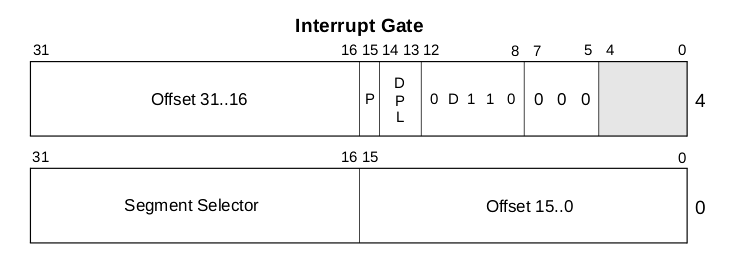
\includegraphics[scale=0.5]{picture/chapt7/interrupt_gate.png}
      \caption{中断描述符的格式}
\end{figure}

\par 根据这个描述信息,我们给出相关的C语言结构体定义:

\begin{lstlisting}[language = C, caption = include/idt.h]
#ifndef INCLUDE_IDT_H_
#define INCLUDE_IDT_H_

#include "types.h"

// 初始化中断描述符表
void init_idt();

// 中断描述符
typedef
struct idt_entry_t {
	uint16_t base_lo;        // 中断处理函数地址 15 ~ 0 位
	uint16_t sel;            // 目标代码段描述符选择子
	uint8_t  always0;        // 置 0 段
	uint8_t  flags;          // 一些标志,文档有解释
	uint16_t base_hi;        // 中断处理函数地址 31 ~ 16 位
}__attribute__((packed)) idt_entry_t;

// IDTR
typedef
struct idt_ptr_t {
	uint16_t limit; 	// 限长
	uint32_t base; 		// 基址
} __attribute__((packed)) idt_ptr_t;

// 寄存器类型
typedef
struct pt_regs_t {
	uint32_t ds;// 用于保存用户的数据段描述符
	uint32_t edi; 		// 从 edi 到 eax 由 pusha 指令压入
	uint32_t esi; 
	uint32_t ebp;
	uint32_t esp;
	uint32_t ebx;
	uint32_t edx;
	uint32_t ecx;
	uint32_t eax;
	uint32_t int_no; 	// 中断号
	uint32_t err_code;  	// 错误代码(有中断错误代码的中断会由CPU压入)
	uint32_t eip;// 以下由处理器自动压入
	uint32_t cs; 		
	uint32_t eflags;
	uint32_t useresp;
	uint32_t ss;
} pt_regs;

// 定义中断处理函数指针
typedef void (*interrupt_handler_t)(pt_regs *);

// 注册一个中断处理函数
void register_interrupt_handler(uint8_t n, interrupt_handler_t h);

// 调用中断处理函数
void idt_handler(pt_regs *regs);

// 声明中断处理函数 0-19 属于 CPU 的异常中断
// ISR:中断服务程序(interrupt service routine)
void isr0(); 		// 0 #DE 除 0 异常 
void isr1(); 		// 1 #DB 调试异常 
void isr2(); 		// 2 NMI 
void isr3(); 		// 3 BP 断点异常 
void isr4(); 		// 4 #OF 溢出 
void isr5(); 		// 5 #BR 对数组的引用超出边界 
void isr6(); 		// 6 #UD 无效或未定义的操作码 
void isr7(); 		// 7 #NM 设备不可用(无数学协处理器) 
void isr8(); 		// 8 #DF 双重故障(有错误代码) 
void isr9(); 		// 9 协处理器跨段操作 
void isr10(); 		// 10 #TS 无效TSS(有错误代码) 
void isr11(); 		// 11 #NP 段不存在(有错误代码) 
void isr12(); 		// 12 #SS 栈错误(有错误代码) 
void isr13(); 		// 13 #GP 常规保护(有错误代码) 
void isr14(); 		// 14 #PF 页故障(有错误代码) 
void isr15(); 		// 15 CPU 保留 
void isr16(); 		// 16 #MF 浮点处理单元错误 
void isr17(); 		// 17 #AC 对齐检查 
void isr18(); 		// 18 #MC 机器检查 
void isr19(); 		// 19 #XM SIMD(单指令多数据)浮点异常

// 20-31 Intel 保留
void isr20();
void isr21();
void isr22();
void isr23();
void isr24();
void isr25();
void isr26();
void isr27();
void isr28();
void isr29();
void isr30();
void isr31();

// 32~255 用户自定义异常
void isr255();

#endif 	// INCLUDE_IDT_H_
\end{lstlisting}

\par 这里的代码很多,不用担心,我们一点一点来解释。

%\begin{lstlisting}[language = C, caption = init/entry.c]
%\end{lstlisting}

%\begin{lstlisting}[language = {[x86masm]Assembler}, caption = gdt/gdt\_s.s]
%\end{lstlisting}
